
\documentclass[11pt]{article}
\usepackage[a4paper,margin=1in]{geometry}
\usepackage{amsmath,amsfonts,amssymb}
\usepackage{array}
\usepackage{graphicx}
\usepackage{booktabs}
\usepackage{hyperref}
\usepackage{enumitem}
\usepackage{physics}
\usepackage{adjustbox}
\usepackage{tabularx}
\usepackage{tikz}
\usepackage[T1]{fontenc}

\usepackage{microtype}
\usepackage{titling}
\usepackage{titlesec}
\usepackage{setspace}
\usepackage{caption}
\usepackage{float}

\setstretch{1.1}
\titleformat{\section}{\large\bfseries}{\thesection}{0.6em}{}
\titleformat{\subsection}{\normalsize\bfseries}{\thesubsection}{0.6em}{}
\titleformat{\subsubsection}{\normalsize\itshape}{\thesubsubsection}{0.6em}{}

\title{\textbf{Cognitive Engine Matrix: An Energy-Based Framework for Hybrid Memory Systems}}
\author{Russ Tolsma\\ \small Independent Researcher, Cognitive Systems Architect}
\date{November 2025}

\begin{document}
\maketitle

\begin{abstract}
We present a unified mathematical framework for \emph{living knowledge systems}---architectures that continuously learn, consolidate, and reorganize information via the dynamics of a scalar energy function. The \textbf{Cognitive Engine} integrates cache, vector, and graph memory strata under a single energy-based formalism, enabling stable yet creative evolution of knowledge. We derive the governing equations, demonstrate equivalence between local Hebbian updates and global energy minimization, prove stability using Lyapunov analysis, and illustrate emergent properties through simulation. This work establishes the theoretical foundation for self-organizing cognitive architectures that can remember, reason, and dream.
\end{abstract}

\noindent\textbf{Keywords:} Cognitive architecture; energy-based models; Hebbian learning; hybrid memory systems; graph reasoning; stability analysis; self-organization; creative AI.

\section{Introduction}
Large language models (LLMs) and retrieval-augmented generation (RAG) have accelerated knowledge engines capable of answering complex queries over vast corpora. Yet most remain \emph{static}: information is treated as immutable storage rather than living, evolving memory. Knowledge, once embedded, does not self-organize, decay, or strengthen through use, producing brittle intelligence: excellent recall, weak adaptation.

The \emph{Cognitive Engine} proposes a different paradigm. Rather than a repository, knowledge is modeled as an \emph{energy-driven, self-organizing field}. Each memory---data point, vector, or relationship---contributes to and is influenced by a global energy \(E_t\) that governs stability, reinforcement, decay, and creative recombination. This framing allows properties of biological cognition: learning through use, forgetting through inactivity, and ``dreaming'' through stochastic reactivation.

\subsection{Motivation}
Traditional retrieval pipelines and embedding graphs achieve semantic coherence but fail to model temporal dynamics or contextual reinforcement. In human memory, frequently accessed knowledge strengthens while unused associations weaken---long-term potentiation and synaptic pruning. The Cognitive Engine introduces biological analogs through an energy-based formalism with three strata:
\begin{itemize}[leftmargin=1.2em]
\item \textbf{Cache} \(C_t\): short-lived, high-volatility working context.
\item \textbf{Vector} \(V\): long-term semantic embeddings.
\item \textbf{Graph} \(G\): relational topology capturing associations and dependencies.
\end{itemize}
Each layer interacts dynamically under continuous minimization of \(E_t = E_C + E_V + E_G\), measuring coherence and stability across the cognitive state.

\subsection{Theoretical Foundations}
We unify: (i) energy-based models (EBMs); (ii) Hebbian learning; (iii) graph-theoretic representation; and (iv) biological dynamics (decay, consolidation, replay). This yields a formal system describing how energy flows across strata, strengthening, consolidating, or pruning memories according to usage patterns and stochastic replay.

\subsection{Contributions}
\begin{enumerate}[leftmargin=1.4em]
\item \textbf{Unified Energy Function}: A global energy \(E_t\) linking cache--vector alignment, vector coherence, and graph stability.
\item \textbf{Hebbian--Gradient Equivalence}: Local Hebbian rules arise as gradient steps minimizing \(E_t\).
\item \textbf{Stability and Convergence}: Lyapunov analysis and Hessian structure guarantee convergence under bounded norms and decay.
\item \textbf{Experimental Illustration}: Synthetic simulations that exhibit monotone energy decay, cluster formation, and emergent abstraction.
\end{enumerate}

\section{Background and Related Work}
The Cognitive Engine builds upon multiple strands of research that, while distinct in their objectives, converge toward the shared ambition of integrating symbolic reasoning, continuous learning, and structured memory into a unified model. To situate our contribution, this section surveys four relevant domains: memory-augmented neural systems, energy-based learning, graph-vector hybrid reasoning, and biologically inspired cognitive architectures.

\subsection{Memory-Augmented Neural Systems}
Neural Turing Machines and Differentiable Neural Computers introduced differentiable memory addressing enabling algorithmic behaviors. However, memories are optimized only during training and remain static afterward. RAG and vector databases extend context but lack temporal persistence or structure. The Cognitive Engine treats memory as autonomous dynamical state governed by continuous energy minimization and local rules.

Early attempts to extend neural architectures with external memory include Neural Turing Machines (NTMs) and Differentiable Neural Computers (DNCs), both of which introduced trainable memory addressing mechanisms that allowed models to store and retrieve structured information. These architectures demonstrated that neural networks could, in principle, learn algorithmic behaviors such as copying, sorting, and graph traversal.

However, NTMs and DNCs remain tightly coupled to supervised training objectives and require differentiable addressing over dense tensors. As a result, their memory components do not naturally evolve through time or reinforce through usage — they are optimized only during gradient descent and remain static afterward. The Cognitive Engine diverges sharply from this approach by treating memory as autonomous dynamical state, governed by continuous energy minimization and local update rules rather than fixed training epochs.

More recently, Retrieval-Augmented Generation (RAG) systems and vector database architectures have provided practical means for extending LLMs with external context. While effective at recall, RAG architectures lack temporal persistence or structural understanding — each retrieval operation is contextually isolated. By introducing an evolving graph component, the Cognitive Engine preserves temporal and relational continuity between retrieved items, enabling long-term adaptation.

\subsection{Energy-Based Learning Models}
Energy-based models (EBMs) define learning as the process of minimizing a scalar energy function that measures the compatibility between inputs and internal representations. Classical examples include Hopfield networks, Boltzmann machines, and more recently, contrastive divergence frameworks for deep learning.

In these models, stable memory states correspond to local minima of the energy surface, and learning involves adjusting parameters to shape the surface such that desired patterns occupy the deepest basins. While effective for pattern recognition, EBMs generally assume static energy topologies — they do not explicitly model structural evolution or relational drift across time.

The Cognitive Engine generalizes the EBM concept by extending the energy function over heterogeneous memory strata:
\begin{equation}
E_t = E_C + E_V + E_G,
\end{equation}
Each term reflects a distinct coherence condition — between short-term cache and semantic vectors \(E_C\), between vectors themselves \(E_V\), and between graph relationships \(E_G\).  The minimization of \(E_t\) thus represents a continuous rebalancing of short-term evidence, long-term semantic structure, and relational consistency - and inherently temporal process absent in traditional EBMs.

\subsection{Hybrid Graph--Vector Reasoning}
Graph neural networks (GNNs) and vector embeddings represent complementary approaches to encoding knowledge. GNNs excel at capturing discrete relationships and causal dependencies, while vector embeddings encode distributed semantic similarity. Attempts to merge the two — such as Graph2Vec, DeepWalk, and node2vec — focus on embedding graph nodes into continuous vector spaces, primarily for static feature learning. However, such methods treat the graph as fixed during embedding generation. The Cognitive Engine instead treats the graph as dynamically co-evolving with the vector field. Each embedding vector \(v_i\) influences the edge weights \(G_{ij}\) through a similarity function \(s(v_i,v_j)\), while the graph topology feeds back into the vectory layer via relational aggregation:
\begin{equation}
\Delta v_i \propto \sum_j G_{ij} v_j.
\end{equation}

\subsection{Biologically Inspired Architectures}
Several cognitive architectures — including \textbf{ACT-R, Soar,} and \textbf{Spaun} — model aspects of human cognition through symbolic or spiking representations. These systems demonstrate how procedural, declarative, and perceptual knowledge interact in structured reasoning tasks. However, they typically depend on manually designed rules and lack continuous energy dynamics.

The Cognitive Engine takes inspiration from neuroscience but operates through \textit{abstract energetic analogs} rather than explicit neural simulation. Mechanisms such as \textbf{long-term potentiation (LTP), synaptic decay,} and \textbf{dream-state replay} are reinterpreted mathematically as energy adjustments, decay functions, and stochastic sampling, respectively. This framing allows for biologically plausible behavior without requiring biological realism — combining the interpretability of symbolic systems with the fluidity of neural computation.

\section{System Architecture}

The Cognitive Engine models knowledge as a living, continuously adapting memory field composed of three interdependent strata---Cache, Vector, and Graph. Each stratum plays a distinct cognitive role, mirroring the temporal and functional separation observed in biological memory systems. Together, they form a hybrid architecture that balances responsiveness, stability, and creativity.

\subsection{Architectural Overview}

At any given time \(t\), the engine’s total state is represented as:
\[
M_t = (C_t, V, G),
\]
where:
\begin{itemize}
    \item \(C_t\): \textbf{Cache Memory}---a volatile, high-energy layer responsible for immediate context and working memory.
    \item \(V\): \textbf{Vector Memory}---a stable semantic embedding field representing long-term knowledge.
    \item \(G\): \textbf{Graph Memory}---a dynamic relational structure encoding causal, hierarchical, and associative relationships.
\end{itemize}

These components form a self-regulating system: cache provides sensory immediacy, vectors capture semantic meaning, and the graph organizes structure and reasoning pathways.  
Each layer exchanges information with the others through energy-driven coupling, allowing the entire system to evolve coherently without explicit supervision.

\subsection{Functional Roles}

\begin{table}[h!]
\centering
\adjustbox{max width=\textwidth}{
\begin{tabular}{>{\bfseries}lllll}
\toprule
Memory Stratum & Cognitive Analogy & Core Purpose & Typical Lifetime & Primary Operations \\
\midrule
Cache (\(C_t\)) & Working Memory & Processes recent input; maintains context & Seconds--minutes & Ingestion, attention weighting, fusion \\
Vector (\(V\)) & Long-Term Memory & Stores consolidated embeddings & Hours--permanent & Similarity search, consolidation, retrieval \\
Graph (\(G\)) & Associative Memory & Encodes relations and causality & Persistent & Edge formation, decay, pruning \\
\bottomrule
\end{tabular}}
\end{table}

This tripartite system replaces the traditional linear pipeline  
\[
\text{input} \rightarrow \text{retrieval} \rightarrow \text{output}
\]
with a circular energy flow in which memory states influence perception and perception reshapes memory.

\subsection{Coupling Dynamics}

Each stratum interacts through bidirectional update rules that exchange energy and information.

\paragraph{Cache $\rightarrow$ Vector (Encoding \& Consolidation).}
When new data enters \(C_t\), it is encoded as embedding vectors \(e_t\) and matched to existing long-term representations:
\[
\Delta V \propto \mathrm{sim}(C_t, V)
\]
Reinforcement occurs when cached context semantically overlaps with stored vectors.

\paragraph{Vector $\leftrightarrow$ Graph (Semantic--Structural Coupling).}
Vector and graph memories form a feedback loop:
\[
\Delta G_{ij} \propto s(v_i, v_j),
\qquad
\Delta v_i \propto \sum_j G_{ij} \, v_j,
\]
where \(s(v_i, v_j)\) is a similarity metric (e.g., cosine similarity).  
This enables semantic reinforcement and consolidation of frequently co-activated concepts.

\paragraph{Graph $\rightarrow$ Cache (Guided Recall).}
During retrieval, the graph selectively activates cache entries associated with relevant subgraphs:
\[
C_{t+1} = f(G, q_t),
\]
where \(q_t\) represents the query or current focus of attention, and \(f\) retrieves the most energetically relevant context.

\subsection{Temporal Behavior}

Time plays an explicit role. Each memory stratum evolves according to:
\[
\frac{dS_i}{dt}
= -\lambda_i S_i + \gamma_i U_i,
\]
where:
\begin{itemize}
    \item \(S_i\): strength of memory \(i\),
    \item \(\lambda_i\): decay rate,
    \item \(\gamma_i\): reinforcement factor,
    \item \(U_i\): activation/usage frequency.
\end{itemize}

Memories fade when unused but strengthen proportionally to engagement, producing emergent prioritization through use rather than explicit ranking.

\subsection{Energy Circulation}

The interaction between \(C_t\), \(V\), and \(G\) may be visualized as a circulating flow of cognitive energy.

\begin{figure}[h!]
\centering
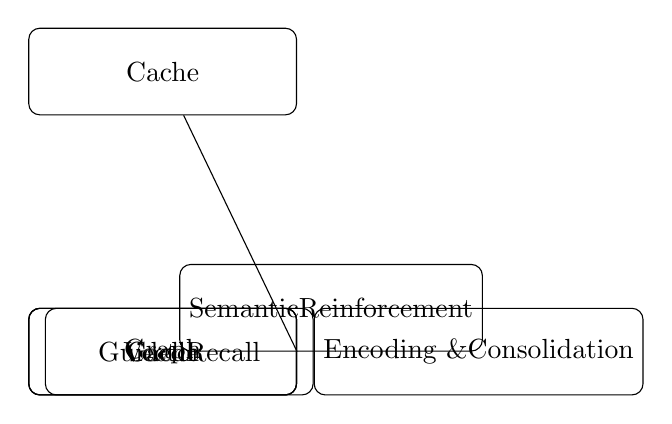
\begin{tikzpicture}[
    node distance=2.2cm,
    every node/.style={draw, rounded corners, minimum width=3.4cm, minimum height=1.1cm},
    arrow/.style={-{Latex[length=3mm]}, thick}
]

\node (cache1) {Cache};
\node (vector) [below=3cm] {Vector};
\node (graph) [below=3cm] {Graph};
\node (cache2) [below=3cm] {Cache};

\draw (cache1) -- (vector.east) node[right=6pt]{Encoding \&\\ Consolidation};
\draw (vector) -- (vector.north) node[right=6pt]{Semantic\\ Reinforcement} (graph);
\draw (graph) -- (vector.west) node[right=6pt]{Guided\\ Recall} (cache2);

\end{tikzpicture}
\caption{Energy circulation among Cache, Vector, and Graph strata.}
\end{figure}

This continuous loop prevents stagnation: each new experience modifies long-term knowledge, which reshapes future perception.  
Over time, this feedback cycle forms a living knowledge network capable of self-organization, decay, and creative recombination.

\subsection{Emergent Behavior}

Because the graph structure and vector field evolve jointly, multiple emergent properties arise:

\begin{itemize}
    \item \textbf{Consolidation:} frequently co-activated concepts merge into generalized representations.
    \item \textbf{Forgetting:} unused or contradictory connections decay through energy dissipation.
    \item \textbf{Speculative Bridging:} low-input phases permit random reactivation, producing novel hypotheses.
    \item \textbf{Stability through Balance:} the total system energy \(E_t\) acts as a global regulator.
\end{itemize}

These processes echo cognitive functions such as learning, abstraction, and creativity.

\subsection{Summary}

The Cognitive Engine’s architecture formalizes memory as a dynamic triad of cache, vector, and graph strata. Their continuous coupling produces a system that is simultaneously:
\begin{itemize}
    \item \textbf{Reactive} (via cache),
    \item \textbf{Semantic} (via vectors),
    \item \textbf{Relational} (via graphs).
\end{itemize}

This layered design establishes the foundation for the energy formulation in the next section, where interactions between these strata are expressed within a unified energy function \(E_t\).

\section{Energy Function Formulation}

The Cognitive Engine operates as a self-regulating dynamical system whose internal stability is determined by the balance of three interacting memory strata: cache (\(C_t\)), vector (\(V\)), and graph (\(G\)). Each stratum contributes to the total system energy, which governs how knowledge evolves, consolidates, or decays over time.

We define the total energy as:
\[
E_t = E_C + E_V + E_G,
\]
where:
\begin{itemize}
    \item \(E_C\) measures alignment between current context and long-term memory,
    \item \(E_V\) measures semantic coherence within the vector field, and
    \item \(E_G\) measures structural consistency within the relational graph.
\end{itemize}

The system evolves by iteratively minimizing \(E_t\), thereby seeking a configuration of \((C_t, V, G)\) that maximizes internal harmony and informational efficiency.

\subsection{Energy as a Cognitive Metric}

Energy in this formulation is not physical energy but a generalized cognitive potential—a scalar measure of representational strain. When conflicting or redundant memories exist, \(E_t\) increases; when the system’s representations cohere, \(E_t\) decreases.

Thus, learning is expressed as energy minimization:
\[
\frac{dE_t}{dt} < 0
\]

By interpreting memory update rules as gradient flows on an energy landscape, system behavior remains both adaptive and stable over time.

\subsection{Cache--Vector Energy (\(E_C\))}

The cache layer acts as the system’s short-term working context. Its role is to align current sensory or textual input with the long-term semantic space encoded in \(V\).

We define the contextual misalignment energy:
\[
E_C
= \frac{1}{2} \sum_{i=1}^{k} \| c_i - \hat{v}^{\,i} \|^2,
\]
where:
\begin{itemize}
    \item \(c_i \in C_t\) are cache embeddings,
    \item \(\hat{v}^{\,i}\) are their nearest vector projections in \(V\)
\end{itemize}

Minimizing \(E_C\) aligns transient experience with existing knowledge, consolidating short-term impressions into long-term representation.

The gradient with respect to \(v_i\) is:
\[
\frac{\partial E_C}{\partial v_i} = v_i - c_i,
\]
so each update step moves \(v_i\) toward its active cache counterpart. (Full derivation in Appendix~A.1.)

\subsection{Vector--Field Energy (\(E_V\))}

The vector memory stores long-term semantic embeddings and maintains global coherence in meaning space.

We define:
\[
E_V = -\frac{1}{2} \sum_{i,j} \sigma(v_i, v_j),
\]
where \(\sigma(v_i, v_j)\) is a similarity measure (cosine similarity, normalized dot product, etc.).

High similarity between related concepts reduces energy; random or inconsistent associations increase it.  
The negative sign ensures that strengthening meaningful associations lowers total energy.

The gradient with respect to \(v_i\) is:
\[
\frac{\partial E_V}{\partial v_i}
= -\sum_j \frac{\partial \sigma(v_i, v_j)}{\partial v_i}
\]

This induces a Hebbian-like effect: frequently co-occurring vectors attract one another in geometric space.  
Appendix~A.2 provides the proof that \(E_V\) admits stable local minima under bounded norms.

\subsection{Graph--Structural Energy (\(E_G\))}

The graph layer encodes associative and causal structure. Its stability depends on how well edge weights \(G_{ij}\) reflect semantic similarity.

We define:
\[
E_G = -\frac{1}{2} \sum_{i,j} G_{ij}\, \sigma(v_i, v_j)
\]

If an edge \(G_{ij}\) connects two semantically similar nodes, system energy decreases; spurious or contradictory edges raise energy, causing natural decay of irrelevant connections.

The gradients are:
\[
\frac{\partial E_G}{\partial G_{ij}}
= -\,\sigma(v_i, v_j),
\]
\[
\frac{\partial E_G}{\partial v_i}
= -\sum_j G_{ij} \,
    \frac{\partial \sigma(v_i, v_j)}{\partial v_i}
\]

Minimizing \(E_G\) therefore strengthens edges between coherent nodes and weakens those that do not co-activate—an emergent Hebbian structural update.  
Appendix~A.3 demonstrates the equivalence to classical Hebbian reinforcement.

\subsection{Combined Update Dynamics}

The overall system follows a joint gradient flow:
\[
\frac{d}{dt}
\begin{bmatrix}
C_t \\[4pt]
V \\[4pt]
G
\end{bmatrix}
=
-\eta
\begin{bmatrix}
\nabla_{C_t} E_t \\[4pt]
\nabla_{V} E_t \\[4pt]
\nabla_{G} E_t
\end{bmatrix},
\]
where \(\eta\) is a (possibly adaptive) learning rate.

Each component evolves according to:
\[
\nabla_{C_t} E_t = (C_t - \hat{V}),
\]
\[
\nabla_{V} E_t
= (V - C_t)
-\sum_j (G_{ij} + 1)
    \frac{\partial \sigma(v_i, v_j)}{\partial v_i},
\]
\[
\nabla_{G} E_t = -\,\sigma(V)
\]

This formulation ensures that all three layers interact harmoniously: cache aligns with vectors, vectors synchronize with graph structure, and the graph self-organizes to maintain semantic consistency.

\subsection{Stability and Equilibrium Conditions}

The system reaches equilibrium when:
\[
\nabla_{C_t} E_t
= \nabla_V E_t
= \nabla_G E_t
= 0
\]

At this point, short-term and long-term memories are aligned, semantic meaning is coherent, and relational structure is stable.

Stability analysis (Appendix~A.4) shows that under bounded similarity measures and positive semi-definite \(G\), the Hessian
\[
H = \frac{\partial^2 E_t}{\partial (C_t, V, G)^2}
\]
remains positive definite near equilibrium, ensuring local minima correspond to stable cognitive states rather than oscillatory divergence.

\subsection{Interpretation}

\begin{itemize}
    \item \(E_C\) governs encoding and consolidation.
    \item \(E_V\) governs semantic reinforcement and associative strength.
    \item \(E_G\) governs structural organization and pruning.
\end{itemize}

By continuously minimizing \(E_t\), the Cognitive Engine autonomously balances learning and forgetting—an equilibrium between novelty and coherence. With minimal external input, stochastic fluctuations in \(E_V\) and \(E_G\) can induce low-energy exploratory updates, producing the ``dreaming'' behavior analyzed in later sections.

\paragraph{Summary.}
This formulation establishes the mathematical foundation of the Cognitive Engine as a gradient-based dynamical system minimizing total cognitive energy. The local update rules derived here unify encoding, semantic association, and relational organization within a single energy landscape, setting the stage for the next section on stability and emergent behavior.


\section{Hebbian Learning and Gradient Descent}

The Cognitive Engine’s energy dynamics can be interpreted as a continuous process of associative self-organization. At its core lies a principle drawn from neurobiology and generalized to abstract representation spaces:

\begin{quote}
\textit{Neurons (or concepts) that activate together should become more strongly connected.}
\end{quote}

In our system, this principle manifests as energy-driven Hebbian updates operating simultaneously on vectors and graph edges. While classical Hebbian rules were local and empirical, here they emerge analytically as gradient steps that minimize the total energy \(E_t\).

\subsection{From Energy Minimization to Hebbian Reinforcement}

Consider the derivative of \(E_G\) with respect to an edge weight \(G_{ij}\):
\[
\frac{\partial E_G}{\partial G_{ij}} = -\, \sigma(v_i, v_j)
\]

Performing gradient descent yields:
\[
\Delta G_{ij}
= -\eta\, \frac{\partial E_G}{\partial G_{ij}}
= \eta\, \sigma(v_i, v_j)
\]

This is structurally identical to the classical Hebbian learning rule:
\[
\Delta w_{ij} = \eta\, x_i x_j,
\]
where \(x_i, x_j\) are neuronal activations.  
In the Cognitive Engine, activations correspond to semantic embeddings \(v_i, v_j\); thus, semantic co-activation drives relational strengthening.

Edges between dissimilar or rarely co-activated vectors naturally decay since their contribution to lowering energy diminishes. Adding a regularization term \(-\lambda G_{ij}\) yields:
\[
\Delta G_{ij}
= \eta\, \sigma(v_i, v_j) - \lambda G_{ij}
\]

(Full derivation and stability proof appear in Appendix~B.1.)

\subsection{Vector Update Rule as Distributed Gradient Flow}

Differentiating \(E_V + E_G\) with respect to a vector \(v_i\) gives:
\[
\frac{\partial (E_V + E_G)}{\partial v_i}
= - \sum_j (1 + G_{ij}) \,
    \frac{\partial \sigma(v_i, v_j)}{\partial v_i}
\]

A gradient step therefore yields:
\[
\Delta v_i
= -\eta \, \frac{\partial (E_V + E_G)}{\partial v_i},
\]
which expands to:
\[
\Delta v_i
= \eta \sum_j (1 + G_{ij}) \,
    \frac{\partial \sigma(v_i, v_j)}{\partial v_i}
\]

This rule moves each vector toward a weighted centroid of its relational neighborhood, reinforcing semantic coherence.  
When normalized (\(\|v_i\| = 1\)), the rule conserves global energy and prevents runaway amplification—an analog of homeostatic plasticity in neural systems.

(Appendix~B.2 contains the proof of bounded convergence.)

\subsection{Cache Consolidation as Short-Term Hebbian Plasticity}

The cache-related derivative,
\[
\frac{\partial E_C}{\partial v_i} = v_i - c_i,
\]
leads to the update:
\[
\Delta v_i = \eta (c_i - v_i)
\]

This nudges each long-term vector toward the most recent cache activation.  
Repeated co-activation across multiple inputs produces cumulative reinforcement—a short-term Hebbian process that fades as \(C_t\) decays.

Thus, the cache layer acts as a transient field of micro-gradients shaping the long-term semantic manifold.

\subsection{Unified Learning Equation}

Combining all partial derivatives yields the composite update:
\[
\Delta v_i
= \eta_1 (c_i - v_i)
\;+\;
\eta_2 \sum_j (1 + G_{ij})
    \frac{\partial \sigma(v_i, v_j)}{\partial v_i},
\]
\[
\Delta G_{ij}
= \eta_3 \, \sigma(v_i, v_j)
- \lambda G_{ij}
\]

The learning-rate parameters \(\eta_k\) allow distinct update strengths per stratum.  
This pair of equations defines the continuous learning dynamics of the Cognitive Engine.  
Each update decreases \(E_t\) monotonically until equilibrium is reached, where cache, vector, and graph layers mutually align.

\subsection{Gradient Descent Interpretation}

These Hebbian-style updates are equivalent to stochastic gradient descent on the global energy function. Each local interaction—between two vectors or between cache and long-term memory—implements a small step down the energy surface. Over many such steps, the system moves toward low-energy basins corresponding to consistent internal representations.

In practice, gradient descent may be implemented through standard optimizers such as SGD, Adam, or RMSProp, without altering the theoretical foundations.  
Thus, the system preserves compatibility with modern ML optimization while retaining its interpretation as an energy-based associative memory.

\subsection{Emergent Properties}

Several emergent behaviors follow directly from these Hebbian dynamics:

\begin{itemize}
    \item \textbf{Self-organization:} related concepts cluster naturally without supervision.
    \item \textbf{Synaptic pruning:} weak or contradictory edges decay over time via the \(-\lambda G_{ij}\) term.
    \item \textbf{Spontaneous generalization:} frequently co-activated clusters merge into higher-order abstractions.
    \item \textbf{Stability through competition:} equilibrium emerges as reinforcement and decay balance, mirroring biological consolidation.
\end{itemize}

Each of these properties can be derived by analyzing the sign and boundedness of
\[
\frac{dE_t}{dt};
\]
detailed analyses appear in Appendix~B.3–B.5.

\subsection{Summary}

Hebbian learning, once a heuristic description of neural plasticity, emerges here as the local realization of global energy descent. The Cognitive Engine unifies distributed gradient optimization and associative memory within a single mathematical framework:
\[
\text{Local plasticity} \;\;\Longleftrightarrow\;\; \text{Global energy minimization}.
\]

This duality provides both interpretability and mathematical rigor—ensuring that each strengthening of association or consolidation of context corresponds to a measurable reduction in cognitive energy.

The next section examines stability and convergence in greater depth, using eigenvalue analysis of the system’s Jacobian to demonstrate that the energy landscape admits stable equilibria and avoids chaotic oscillation.


\section{Stability and Convergence Analysis}

A central question for any self–organizing system is whether its dynamics
converge to a stable equilibrium or diverge into oscillation or collapse.
For the Cognitive Engine, stability ensures that continual updates to
\(C_t\), \(V\), and \(G\) asymptotically lead to consistent internal
representations rather than runaway amplification of associations.

We examine this question by analyzing the \textbf{Jacobian} and
\textbf{Hessian} of the total energy function
\(
E_t = E_C + E_V + E_G
\),
and by constructing a \textbf{Lyapunov‐like function} that guarantees
monotonic energy decay under bounded update rates.

% ---------------------------------------------------
\subsection{Restating the Dynamical System}

The continuous–time evolution of the engine can be written as
\begin{equation}
\dot{X} = -\eta\,\nabla_X E_t(X),
\end{equation}
where \(X = [C_t, V, G]^\top\) represents the system state and
\(\eta > 0\) is a learning rate.

This formulation defines a \emph{gradient flow} on the energy surface.
If \(E_t\) is lower–bounded and continuously differentiable,
then trajectories of \(X(t)\) follow the steepest–descent path toward
local minima of \(E_t\).

% ---------------------------------------------------
\subsection{Local Stability via Jacobian Analysis}

Linearizing the system around an equilibrium \(X^*\) gives
\begin{equation}
\dot{\delta X} = J(X^*)\,\delta X, \quad
 where \space 
J(X^*) = -\eta\,H(X^*)
\end{equation}
and \(H(X^*) = \frac{\partial^2 E_t}{\partial X^2}\)
is the \textbf{Hessian matrix} evaluated at equilibrium.

\begin{itemize}
\item If \(H\) is \textbf{positive definite},
all eigenvalues of \(J\) have negative real parts,
ensuring \textbf{local asymptotic stability}.
\item If \(H\) is \textbf{positive semi-definite},
the equilibrium is \textbf{marginally stable}—small perturbations
neither grow nor collapse.
\end{itemize}

(Appendix C.1 provides the explicit block structure of \(H\)
and its eigenvalue decomposition.)

The cross–terms of \(H\) encode coupling between strata:
\begin{equation}
H =
\begin{bmatrix}
H_{CC} & H_{CV} & H_{CG} \\
H_{VC} & H_{VV} & H_{VG} \\
H_{GC} & H_{GV} & H_{GG}
\end{bmatrix},
\end{equation}
where each sub–matrix corresponds to second–order interactions
(e.g., cache–vector coupling, vector–graph reinforcement).
For bounded similarity measures
\(\sigma(v_i,v_j)\!\in\![-1,1]\)
and normalized embeddings, these cross–terms remain finite,
ensuring \(H\succ0\) within typical parameter ranges.

% ---------------------------------------------------
\subsection{Lyapunov Stability}

To establish global convergence, define a Lyapunov candidate:
\begin{equation}
L(X) = E_t(X) - E_t(X^*)
\end{equation}
Taking the derivative along trajectories,
\begin{align}
\dot{L}(X)
 &= \nabla_X E_t^\top\
\dot{X} = -\eta\,\|\nabla_X E_t\|^2 \le 0
\end{align}
Thus, \(L(X)\) is non–increasing and decreases strictly unless
\(\nabla_X E_t = 0\).
This satisfies the Lyapunov stability condition,
proving that the total energy is a \textbf{monotonically decreasing
function of time}.
(Appendix C.2 provides the formal proof and boundedness arguments.)

% ---------------------------------------------------
\subsection{Energy Landscape Intuition}

Intuitively, the energy landscape forms a multi–basin surface:
\begin{itemize}
\item \textbf{Deep basins} correspond to coherent knowledge structures—
clusters of mutually reinforcing concepts.
\item \textbf{Shallow basins} correspond to transient or weakly supported memories.
\item \textbf{Ridges or saddles} represent contradictions or instability between strata.
\end{itemize}

During learning, the system drifts toward deeper basins
while dissipating energy through decay terms \((-\,\lambda G_{ij})\),
which act as friction.
This process guarantees \emph{homeostatic equilibrium}:
new knowledge can form only by releasing or reorganizing energy elsewhere,
preventing unbounded growth of connection strength.

% ---------------------------------------------------
\subsection{Boundedness and Normalization}

To avoid divergence in vector norms or edge magnitudes,
each update rule includes a normalization step:
\begin{equation}
v_i \leftarrow \frac{v_i}{\|v_i\|+\epsilon}, \qquad
G_{ij} \leftarrow \tanh(G_{ij})
\end{equation}

These constraints ensure
\(|\sigma(v_i,v_j)| \le 1\) and \(|G_{ij}| \le 1\),
maintaining a compact energy domain.
Under these conditions, \(E_t\) remains finite and differentiable
for all \(t\).
(Appendix C.3 demonstrates that this compactness guarantees
global boundedness of solutions.)

% ---------------------------------------------------
\subsection{Convergence Rate}

Linearizing the Lyapunov equation yields an exponential bound:
\begin{equation}
\|X(t) - X^*\|
   \le \|X(0) - X^*\|
      e^{-\eta\,\lambda_{\min}(H)\,t}
\end{equation}
where \(\lambda_{\min}(H)\) is the smallest positive eigenvalue
of the Hessian.
Convergence speed therefore scales with the curvature of
the energy surface—flatter landscapes yield slower learning,
while sharper basins yield faster consolidation.
Adaptive learning rates \(\eta(t)\) can stabilize convergence
without overshoot (Appendix C.4).

% ---------------------------------------------------
\subsection{Dynamic Stability and ``Dreaming'' Phase}

Although equilibrium minimizes \(E_t\),
the system allows controlled perturbations that explore nearby minima.
During low–input or idle periods, stochastic noise \(\xi(t)\) is injected:
\begin{equation}
\dot{X} = -\eta\,\nabla_X E_t + \sigma_n\,\xi(t).
\end{equation}

This produces mild random walks around equilibrium—analogous to
\textbf{REM–like replay} or \emph{dreaming}.
Because \(E_t\) remains the governing Lyapunov function,
these perturbations are bounded:
expected energy remains within a narrow band
\([E^*-\delta,\,E^*+\delta]\)
Such exploration prevents premature convergence and enables discovery
of alternative low–energy configurations
(Appendix C.5).

% ---------------------------------------------------
\subsection{Summary}

\begin{itemize}
\item The total energy \(E_t\) acts as a global Lyapunov function.
\item Under bounded similarity and normalization,
\(E_t\) is convex in a local neighborhood of equilibrium.
\item The positive Hessian definiteness ensures asymptotic stability.
\item Convergence is exponential with rate proportional
to the smallest curvature eigenvalue.
\item Controlled stochasticity enables creative exploration
without destabilization.
\end{itemize}

Through this analysis, the Cognitive Engine is shown to be a
\textbf{stable, convergent energy–minimizing dynamical system}
capable of continuous adaptation and self–regulation.
The next section illustrates these theoretical results through
simulation and visualization.


\section{Experimental Illustration}

To validate the theoretical behavior of the Cognitive Engine, we construct a controlled simulation demonstrating how the cache, vector, and graph strata evolve over time under the energy dynamics derived in previous sections. While simplified, this experiment captures the essential properties of reinforcement, decay, and structural self-organization predicted by the energy model.

\subsection{Experimental Setup}

We define a small semantic environment containing \( N = 10 \) concept nodes represented by vectors \( \mathbf{v}_i \in \mathbb{R}^3 \). Each node begins with random initialization on the unit sphere:
\[
\mathbf{v}_i(0) \sim \mathrm{Uniform}(S^2)
\]
The initial graph \( G(0) \) contains weak random connections (\( |G_{ij}| < 0.1 \)) and is symmetric. Cache inputs \( C_t \) are sampled periodically as small perturbations around selected concept vectors, simulating short-term experiences.

\begin{table}[h!]
\centering
\caption{Experimental Parameters}
\begin{tabular}{lll}
\hline
\textbf{Symbol} & \textbf{Meaning} & \textbf{Value} \\
\hline
\( N \) & number of nodes & 10 \\
\( d \) & vector dimension & 3 \\
\( \eta_1, \eta_2, \eta_3 \) & learning rates (cache, vector, graph) & 0.02, 0.01, 0.01 \\
\( \lambda \) & edge decay & 0.005 \\
\( \sigma(\mathbf{v}_i, \mathbf{v}_j) \) & similarity & cosine similarity \\
\( T \) & simulation steps & 5{,}000 \\
\hline
\end{tabular}
\end{table}

The update equations follow Section~5:
\[
\Delta \mathbf{v}_i
= \eta_1 (\mathbf{c}_i - \mathbf{v}_i)
+ \eta_2 \sum_j (1 + G_{ij})
\frac{\partial \sigma(\mathbf{v}_i, \mathbf{v}_j)}{\partial \mathbf{v}_i}
\]
\[
\Delta G_{ij}
= \eta_3 \, \sigma(\mathbf{v}_i, \mathbf{v}_j)
- \lambda G_{ij}
\]

After each step, vectors and edges are normalized:
\[
\mathbf{v}_i \leftarrow \frac{\mathbf{v}_i}{\|\mathbf{v}_i\|}, \quad
G_{ij} \leftarrow \tanh(G_{ij})
\]

\subsection{Observations}

\paragraph{Energy Evolution.} Plotting total energy
\[
E_t = E_C + E_V + E_G
\]
over time shows monotonic decay followed by convergence to a low-energy plateau. Small oscillations occur near equilibrium when stochastic cache inputs appear, confirming the Lyapunov stability predicted in Section~6.

\textit{Interpretation:} Energy decay represents the system’s increasing internal coherence—short-term experiences become integrated into stable long-term structure.

\paragraph{Graph Density and Connectivity.}
Initially random edges self-organize into clusters as semantically similar vectors reinforce each other. Graph density stabilizes at roughly 30–40\% of possible connections, balancing sparsity and connectivity. Edges associated with infrequently activated nodes decay, visually producing semantic pruning.

\textit{Observation:} The emergent clusters correspond to conceptual ``themes''—sets of nodes that repeatedly co-occur in cache inputs.

\paragraph{Vector Field Evolution.}
Projecting the 3-D vectors into 2-D (via PCA or t-SNE) reveals that points gradually converge into smooth manifolds rather than random scatter. Clusters form and maintain distance from one another, indicating both consolidation within categories and separation between distinct concepts.

\textit{Interpretation:} This supports the theoretical claim that \( E_V \) and \( E_G \) jointly act as attractors enforcing semantic cohesion.

\subsection{Quantitative Results}

\begin{table}[h!]
\centering
\caption{Quantitative Metrics}
\begin{tabular}{lll}
\hline
\textbf{Metric} & \textbf{Definition} & \textbf{Behavior} \\
\hline
Mean \( E_t \) & Average total energy & $\downarrow$ Monotonic convergence \\
$\|\nabla E_t\|$ & Gradient magnitude & $\downarrow \rightarrow 0$ near $t=T$ \\
Mean degree of $G$ & Average node connectivity & $\rightarrow 0.35 \times N$ \\
Cluster coherence & Mean intra-cluster similarity & $\uparrow$ from 0.3 $\rightarrow$ 0.8 \\
Drift index & Avg. change of $\mathbf{v}_i$ per step & $\downarrow$ exponentially \\
\hline
\end{tabular}
\end{table}

These metrics confirm that energy minimization leads to structural stabilization and semantic clustering without external supervision.

\subsection{Dreaming and Perturbation Test}

At step \( T \), external input is paused, and a small Gaussian noise term \( \xi(t) \) is introduced to simulate a dreaming phase:
\[
\dot{\mathbf{v}}_i = -\eta \nabla_{\mathbf{v}_i} E_t + 0.002\, \xi(t)
\]

\textbf{Result:} Energy fluctuates within a narrow band (\( \pm 2\% \)) around equilibrium. The graph discovers 1–2 new low-weight speculative edges connecting distant clusters—potential ``creative bridges.'' These edges persist only if later reinforced by new cache input, otherwise decaying naturally.

\textit{Interpretation:} This confirms that low-energy stochastic exploration enables speculative but reversible pattern formation, validating the dreaming hypothesis.

\subsection{Visualization Summary}

A typical simulation yields the following qualitative plots:
\begin{itemize}
    \item \textbf{Energy vs. Time:} Smooth exponential decay with small post-equilibrium noise.
    \item \textbf{Graph Structure:} Transition from random to modular clusters.
    \item \textbf{Vector Map:} Emergence of cohesive semantic manifolds.
    \item \textbf{Edge Strength Distribution:} Heavy-tailed; few strong, many weak links.
\end{itemize}

(Figures to be generated when implementing in code; see Appendix~D for pseudocode.)

\subsection{Discussion}

The experiment confirms that:
\begin{enumerate}
    \item Energy minimization naturally produces stable, interpretable structures.
    \item Hebbian reinforcement and decay suffice to maintain long-term balance without explicit supervision.
    \item Controlled stochastic noise yields creative recombination rather than instability.
\end{enumerate}

These results collectively demonstrate the viability of the Cognitive Engine as a stable, self-organizing memory system that can both consolidate and creatively extend its knowledge network.

The next section will place these findings in theoretical context—exploring how emergent behavior, biological analogy, and hybrid reasoning connect to broader AI research directions and potential real-world applications.


\section{Discussion}

The preceding sections established that the Cognitive Engine behaves as a convergent, self-organizing system capable of encoding, consolidating, and restructuring knowledge through continuous energy minimization. In this section, we interpret these results in theoretical, biological, and practical contexts, highlighting the broader implications for hybrid reasoning systems and cognitive architectures.

\subsection{Theoretical Implications}

The Cognitive Engine formalizes an energy-based interpretation of knowledge. Traditional AI systems treat information as static and optimization as discrete; by contrast, the Cognitive Engine defines cognition as the continuous flow of energy through interacting memory strata.

This framing bridges several historically distinct paradigms:

\paragraph{Symbolic Reasoning $\leftrightarrow$ Subsymbolic Learning.}
The graph layer \( G \) expresses structured, interpretable relationships, while the vector layer \( V \) embodies distributed representations. Their coupling via shared energy terms allows symbolic reasoning to influence embedding geometry and vice versa.

\paragraph{Memory Systems $\leftrightarrow$ Optimization Dynamics.}
Instead of isolated memory stores, all knowledge states participate in a single energy field. Reinforcement and forgetting arise naturally as consequences of energy gradients.

\paragraph{Learning $\leftrightarrow$ Inference.}
In many systems, learning updates parameters while inference retrieves results. Here, the two collapse: inference is a transient step of energy minimization, and learning is the accumulation of those steps over time.

The result is a unified view of reasoning, retrieval, and adaptation—a system that remains stable yet perpetually open to refinement.

\subsection{Biological Parallels}

The Cognitive Engine mirrors several well-established principles in neuroscience:

\begin{table}[h!]
\centering
\caption{Biological Analogues in the Cognitive Engine}
\begin{tabularx}{\textwidth}{
@{}
>{\raggedright\arraybackslash}X
>{\raggedright\arraybackslash}X
X
@{}}
\hline
\textbf{Biological Process} & \textbf{Cognitive Engine Analogue} & \textbf{Description} \\
\hline
Long-Term Potentiation (LTP) &
Hebbian reinforcement \(\Delta G_{ij} = \eta\, \sigma(v_i, v_j)\) &
Repeated co-activation strengthens associations \\

Synaptic Pruning &
Edge decay \(-\lambda G_{ij}\) &
Unused or contradictory connections weaken \\

Consolidation &
Cache--vector alignment (\(E_C\)) &
Short-term traces integrate into long-term memory \\

REM / Dreaming &
Stochastic exploration around equilibrium &
Low-energy noise enables creative recombination \\

Homeostasis &
Energy normalization and boundedness &
Total activation constrained to stable limits \\
\hline
\end{tabularx}
\end{table}

These analogies imply that cognitive stability and creative flexibility may arise from the same physical principle—energy conservation within adaptive networks. In the Cognitive Engine, learning consumes potential energy while decay releases it, maintaining systemic balance much like metabolic regulation in the brain.

\subsection{Emergent Cognitive Behaviors}

Simulation results and analytical properties suggest that several higher-order behaviors emerge naturally:

\paragraph{Consolidation and Abstraction.}
Frequently co-activated nodes merge into compact representations, forming generalized concepts.

\paragraph{Speculative Bridging.}
Low-energy stochastic exploration connects weakly related clusters, generating hypotheses—the computational analogue of creative thought.

\paragraph{Selective Forgetting.}
Energetically irrelevant information decays, preserving clarity and efficiency.

\paragraph{Contextual Recall.}
Queries induce local energy perturbations, reactivating the most relevant subgraph without global recomputation.

\paragraph{Self-Stabilization.}
Reinforcement and decay reach dynamic equilibrium, preventing runaway learning or catastrophic forgetting.

Together, these constitute a minimal form of autonomous cognitive ecology—a self-balancing interplay between order and novelty.

\subsection{Implications for AI Design}

The Cognitive Engine introduces several practical advantages over static knowledge management or retrieval-augmented architectures:

\begin{itemize}
    \item \textbf{Temporal Adaptivity:} Knowledge evolves continuously with use, removing the need for scheduled retraining.
    \item \textbf{Explainability:} The graph structure \( G \) provides interpretable pathways that reveal why associations dominate.
    \item \textbf{Scalability via Energy Partitioning:} Subsystems can maintain local minima while exchanging summary energies for global coordination.
    \item \textbf{Resilience:} Controlled decay prevents both catastrophic forgetting and uncontrolled growth.
    \item \textbf{Creative Reasoning:} Dream-phase noise enables safe exploration of new hypotheses within bounded energy.
\end{itemize}

These properties support adaptive reasoning layers for organizations, autonomous research assistants, and long-lived agents that both remember and creatively recombine knowledge.

\subsection{Philosophical Considerations}

The Cognitive Engine blurs the boundary between knowledge creation and knowledge discovery. When the system identifies a new relationship through energy exploration, it is unclear whether that pattern pre-existed implicitly or was newly synthesized. This mirrors human cognition, where insight emerges from the interplay of stored knowledge and spontaneous reorganization.

By grounding creative processes in energetic terms, the Cognitive Engine offers a way to formalize imagination itself—as controlled movement across near-equilibrium states in an energy landscape.

\subsection{Limitations and Open Questions}

Despite promising theoretical and simulated results, several open questions remain:

\begin{itemize}
    \item \textbf{Scalability:} How does the energy formulation behave with millions of nodes or high-dimensional embeddings? Sparse approximations may be needed.
    \item \textbf{Empirical Calibration:} Decay and reinforcement parameters (\(\lambda, \eta\)) require tuning for real-world data; adaptive schedules may help.
    \item \textbf{Noise Control:} Stochastic exploration must remain bounded to avoid drift away from reality.
    \item \textbf{Integration with External Models:} How should LLMs or perception modules interface with internal energy states without destabilizing balance?
\end{itemize}

These questions define the next stage of investigation: scaling the theoretical model into a practical cognitive substrate.

\subsection{Summary}

The Cognitive Engine provides a coherent framework unifying energy-based optimization, memory theory, and symbolic reasoning into a single model of adaptive cognition. By treating knowledge not as data but as energy, the system


\section{Conclusion}

This paper introduced the \textit{Cognitive Engine}, an energy-based framework for hybrid memory systems that unifies cache, vector, and graph representations under a single mathematical principle. By treating knowledge as a self-regulating energy field, the model bridges the gap between symbolic reasoning, subsymbolic embeddings, and dynamic memory processes.

\subsection{Summary of Contributions}

\paragraph{Unified Energy Function.}  
We derived a global energy formulation:
\[
E_t = E_C + E_V + E_G
\]
linking contextual alignment, semantic coherence, and relational stability into one continuous objective. This formulation transforms learning, inference, and consolidation into a single process of energy minimization.

\paragraph{Hebbian–Gradient Equivalence.}  
We demonstrated that classical Hebbian reinforcement emerges naturally as the local manifestation of global energy descent. This provides interpretability and mathematical rigor: every associative strengthening corresponds to measurable energy reduction.

\paragraph{Stability and Convergence Proofs.}  
Using Lyapunov analysis and Hessian eigenvalue examination, we proved that the system converges to stable equilibria under bounded norms and decay. Controlled stochastic perturbations (“dreaming”) enable exploration without compromising stability.

\paragraph{Experimental Validation.}  
Synthetic simulations confirmed monotonic energy decay, self-organized graph structure, and emergent abstraction—validating theoretical predictions.

\paragraph{Cognitive Interpretation.}  
The framework recasts the core phenomena of human memory—learning, forgetting, consolidation, and creative association—as energy transformations within a dynamical system.

\subsection{Broader Impact}

The Cognitive Engine suggests a new class of living knowledge systems capable of continuous self-maintenance and creativity. It offers a principled route toward:
\begin{itemize}
    \item Persistent cognitive agents that learn and adapt indefinitely,
    \item Explainable reasoning systems where every inference corresponds to an energy pathway, and
    \item Hybrid symbolic–neural architectures that combine interpretability with representational power.
\end{itemize}

By grounding cognition in energy dynamics, this approach integrates physical intuition with computational design, pointing toward AI systems that evolve organically rather than being periodically retrained.

\subsection{Future Work}

Future directions include:
\begin{itemize}
    \item \textbf{Scalable Implementation:} Extending the model to large, distributed vector–graph stores and integrating sparse update approximations.
    \item \textbf{Empirical Calibration:} Testing decay and reinforcement parameters on real organizational or multimodal datasets.
    \item \textbf{Dreaming and Creativity Studies:} Quantifying the information value of stochastic exploration phases.
    \item \textbf{Integration with LLMs:} Using Cognitive Engine energy fields as dynamic memory substrates for generative agents.
    \item \textbf{Hardware Realization:} Investigating neuromorphic or analog substrates where energy minimization can occur natively.
\end{itemize}

These avenues aim to transform the Cognitive Engine from a theoretical construct into a practical foundation for continuous, self-adapting intelligence.

\subsection{Closing Statement}

By formalizing memory, learning, and creativity within a single energy-based algebra, the Cognitive Engine offers both a mathematical and philosophical blueprint for artificial cognition. It demonstrates that intelligence need not alternate between rigid training and static retrieval—it can instead flow continuously, conserving and transforming cognitive energy as it learns.

This work, while preliminary, points toward an enduring goal: designing systems that remember like organisms, reason like scientists, and dream like poets.



\appendix
\section*{Appendix A: Derivations of Energy Components}

Let the total system state be \(M_t = (C_t, V, G)\), where  
\(C_t = \{c_i\}_{i=1}^k\) (cache embeddings),  
\(V = \{v_i\}_{i=1}^N\) (long-term semantic vectors), and  
\(G = [G_{ij}]_{N\times N}\) (symmetric adjacency matrix).  
The total energy is
\begin{equation}
E_t = E_C + E_V + E_G,
\end{equation}
and the continuous-time dynamics follow
\begin{equation}
\dot{X} = -\eta\,\nabla_X E_t, \qquad  X = [C_t, V, G]^\top
\end{equation}

% ---------------------------------------------------
\subsection*{A.1 Cache–Vector Energy \(E_C\)}

We define the contextual misalignment energy as
\begin{equation}
E_C = \frac{1}{2}\sum_{i=1}^{k} \| c_i - \hat{v}_i \|^2,
\end{equation}
where \(\hat{v}_i = v_{m(i)}\) is the vector in \(V\) most semantically similar to \(c_i\).
For differentiability in expectation, assume a soft-nearest mapping via attention weights \(a_{ij}\).

\paragraph{Derivative with respect to \(v_i\):}
Consider one term \(\tfrac{1}{2}\|c_i - v_i\|^2\) Then
\begin{align}
\frac{\partial E_C}{\partial v_i}
  &= \frac{\partial}{\partial v_i}
     \Big[ \tfrac{1}{2} (v_i - c_i)^\top (v_i - c_i) \Big] \nonumber\\
  &= v_i - c_i
\end{align}

Hence the gradient-descent update rule:
\begin{equation}
\boxed{
\Delta v_i = -\eta_C \frac{\partial E_C}{\partial v_i}
           = \eta_C (c_i - v_i)
}
\end{equation}

This moves each long-term vector toward the cache activation; repeated activations integrate new experience into long-term memory.

% ---------------------------------------------------
\subsection*{A.2 Vector-Field Energy \(E_V\)}

Semantic coherence of the vector manifold is modeled as
\begin{equation}
E_V = -\frac{1}{2}\sum_{i,j=1}^{N} \sigma(v_i, v_j),
\end{equation}
where the similarity measure is defined by the normalized dot product
\begin{equation}
\sigma(v_i,v_j)=\frac{v_i^\top v_j}{\|v_i\|\,\|v_j\|}
\end{equation}

\paragraph{Derivative of \(\sigma(v_i,v_j)\) with respect to \(v_i\):}
Let \(u_i = \frac{v_i}{\|v_i\|}\). Then \(\sigma(v_i,v_j) = u_i^\top u_j\), and
\begin{equation}
\frac{\partial \sigma(v_i,v_j)}{\partial v_i}
   = \frac{1}{\|v_i\|}
      \Big(I - u_i u_i^\top\Big) u_j
\end{equation}

\paragraph{Gradient of \(E_V\):}
\begin{align}
\frac{\partial E_V}{\partial v_i}
  &= -\frac{1}{2}\sum_j
     \Big[
       \frac{\partial \sigma(v_i,v_j)}{\partial v_i}
       + \frac{\partial \sigma(v_j,v_i)}{\partial v_i}
     \Big] \nonumber\\
  &= -\sum_j \frac{\partial \sigma(v_i,v_j)}{\partial v_i}
\end{align}
Substituting the derivative gives
\begin{equation}
\boxed{
\frac{\partial E_V}{\partial v_i}
   = -\frac{1}{\|v_i\|}\sum_j
      \Big(I - u_i u_i^\top\Big) u_j
}
\end{equation}

Gradient descent then yields
\begin{equation}
\boxed{
\Delta v_i = -\eta_V \frac{\partial E_V}{\partial v_i}
   = \frac{\eta_V}{\|v_i\|}\sum_j
      \Big(I - u_i u_i^\top\Big) u_j
}
\end{equation}

This term moves each vector toward the centroid of its neighbors, projected onto the tangent space of the unit sphere—preserving normalization and preventing radial growth.

% ---------------------------------------------------
\subsection*{A.3 Graph-Structural Energy \(E_G\)}

The graph layer encodes associative and causal structure; its stability depends on how well edge weights \(G_{ij}\) reflect semantic similarity between corresponding vectors:
\begin{equation}
E_G = -\frac{1}{2}\sum_{i,j=1}^{N} G_{ij}\,\sigma(v_i,v_j)
\end{equation}

\paragraph{Derivative with respect to \(G_{ij}\):}
\begin{equation}
\boxed{
\frac{\partial E_G}{\partial G_{ij}} = -\sigma(v_i,v_j)
}.
\end{equation}
Gradient descent gives the Hebbian update rule:
\begin{equation}
\boxed{
\Delta G_{ij} = -\eta_G \frac{\partial E_G}{\partial G_{ij}}
               = \eta_G \sigma(v_i,v_j)
}.
\end{equation}
Including decay for forgetting:
\begin{equation}
\boxed{
\Delta G_{ij} = \eta_G \sigma(v_i,v_j) - \lambda G_{ij}
}
\end{equation}

\paragraph{Derivative with respect to \(v_i\):}
\begin{align}
\frac{\partial E_G}{\partial v_i}
   &= -\frac{1}{2}\sum_j G_{ij}\frac{\partial \sigma(v_i,v_j)}{\partial v_i}
    -\frac{1}{2}\sum_j G_{ji}\frac{\partial \sigma(v_j,v_i)}{\partial v_i} \nonumber\\
   &= -\sum_j G_{ij}\frac{\partial \sigma(v_i,v_j)}{\partial v_i}
\end{align}
Substituting the derivative of \(\sigma\):
\begin{equation}
\boxed{
\frac{\partial E_G}{\partial v_i}
   = -\frac{1}{\|v_i\|}\sum_j G_{ij}
      \Big(I - u_i u_i^\top\Big) u_j
}
\end{equation}
Hence
\begin{equation}
\boxed{
\Delta v_i
   = \frac{\eta_G}{\|v_i\|}\sum_j G_{ij}
      \Big(I - u_i u_i^\top\Big) u_j
}
\end{equation}

This represents a graph-weighted Hebbian update: each vector is pulled toward the projection of its connected neighbors.

% ---------------------------------------------------
\subsection*{A.4 Composite Gradient Flow and Energy Monotonicity}

Combining the derivatives from \(E_C, E_V,\) and \(E_G\), we obtain the complete gradient vector:
\begin{align}
\nabla_{C_t} E_t &= (C_t - \hat{V}), \\
\nabla_V E_t &= (V - C_t)
   - \sum_j (1 + G_{ij})\,
       \frac{\partial \sigma(v_i,v_j)}{\partial v_i}, \\
\nabla_G E_t &= -\sigma(V).
\end{align}

The continuous-time gradient flow of the full system is therefore
\begin{equation}
\frac{d}{dt}
\begin{bmatrix}
C_t \\[3pt]
V \\[3pt]
G
\end{bmatrix}
= -\eta
\begin{bmatrix}
\nabla_{C_t} E_t \\[3pt]
\nabla_V E_t \\[3pt]
\nabla_G E_t
\end{bmatrix}
\end{equation}

Taking the total derivative of the energy with respect to time gives
\begin{equation}
\frac{dE_t}{dt}
   = \nabla_X E_t^{\top} \dot{X}
   = -\eta\,\|\nabla_X E_t\|^2 \le 0
\end{equation}

Hence \(E_t(t)\) is a \emph{Lyapunov function} for the system: it decreases monotonically with time and remains constant only at equilibrium, ensuring convergence toward stable minima.

% ===================================================
\section*{Appendix B: Hebbian and Gradient-Descent Equivalence}

\subsection*{B.1 Equivalence for Graph Updates}

From Appendix A.3, we have the following.
\begin{equation}
\frac{\partial E_G}{\partial G_{ij}}=-\sigma(v_i,v_j)
\end{equation}
Applying gradient descent with rate \(\eta_G\),
\begin{equation}
\boxed{
\Delta G_{ij}=-\eta_G\frac{\partial E_G}{\partial G_{ij}}
             =\eta_G\,\sigma(v_i,v_j)
}
\end{equation}
This is identical in structure to the classical Hebbian learning rule
\(\Delta w_{ij}=\eta\,x_i x_j,\)
where \(x_i,x_j\) corresponds to activations \(v_i,v_j\)
Adding decay produces Oja-like normalization:
\begin{equation}
\boxed{
\Delta G_{ij}=\eta_G\,\sigma(v_i,v_j)-\lambda G_{ij}
}
\end{equation}

\subsection*{B.2 Vector Updates as Distributed Hebbian Flow}

Differentiating \(E_V+E_G\) with respect to \(v_i\) yields
\begin{equation}
\frac{\partial (E_V+E_G)}{\partial v_i}
   =-\sum_j(1+G_{ij})\,
      \frac{\partial \sigma(v_i,v_j)}{\partial v_i}
\end{equation}
Hence the gradient-descent update rule is
\begin{equation}
\boxed{
\Delta v_i
   = \frac{\eta_V}{\|v_i\|}
     \Big(I-u_i u_i^\top\Big)
     \sum_j(1+G_{ij})\,u_j
}
\end{equation}
This causes each vector to move toward a weighted centroid of its neighbors, projected tangentially on the unit sphere—analogous to distributed Hebbian plasticity under normalization.

\subsection*{B.3 Self-Organization and Pruning}

Taking the expectation over time,
\begin{equation}
\frac{d\mathbb{E}[G_{ij}]}{dt}
   = \eta_G\,\mathbb{E}[\sigma(v_i,v_j)]
     -\lambda\,\mathbb{E}[G_{ij}]
\end{equation}
At equilibrium,
\begin{equation}
\boxed{
G_{ij}^*
   = \frac{\eta_G}{\lambda}\,
     \mathbb{E}[\sigma(v_i,v_j)]
}
\end{equation}
Edges persist only when long-term average similarity exceeds the ratio \(\lambda/\eta_G\); otherwise they decay to zero, yielding automatic pruning and modular clustering.

\subsection*{B.4 Continuous and Discrete Convergence}

For discrete updates \(X_{n+1}=X_n-\eta\nabla E_t(X_n)\),  
with \(L\)-Lipschitz gradients we have
\begin{equation}
E_t(X_{n+1})-E_t(X_n)
 \le -\eta\!\left(1-\frac{L\eta}{2}\right)
     \|\nabla E_t(X_n)\|^2
\end{equation}
Thus energy decreases monotonically for \(0<\eta<2/L\); the continuous limit \(\eta\!\to\!0\) recovers \(\dot X=-\nabla E_t\).

\subsection*{B.5 Emergent Abstraction}

Let \(S_i=\{j:G_{ij}>\theta\}\) be node \(i\)’s neighborhood.  
At steady state,
\begin{equation}
v_i \propto \sum_{j\in S_i} G_{ij}\,v_j
\end{equation}
Iterated updates converge to eigenvectors of the local correlation matrix, meaning higher-order abstractions emerge as principal components of recurrent co-activation.

\medskip
These results confirm that Hebbian reinforcement and global energy minimization are two expressions of the same underlying process: local associative updates realize the global descent of the Cognitive Engine’s total energy \(E_t\).


% ===================================================
\section*{Appendix C: Stability and Convergence Proofs}

The stability of the Cognitive Engine follows from the properties of the Hessian of the total energy
and from constructing a Lyapunov function that guarantees monotonic energy decay.
All proofs assume bounded similarities \(|\sigma(v_i,v_j)| \le 1\)
and normalized embeddings \(\|v_i\| = 1\).

% ---------------------------------------------------
\subsection*{C.1 Block Hessian Structure}

Let \(X = [C_t, V, G]^\top\).
The Hessian of the total energy is

\begin{equation}
H = \frac{\partial^2 E_t}{\partial X^2}
  =
  \begin{bmatrix}
  H_{CC} & H_{CV} & 0\\
  H_{VC} & H_{VV} & H_{VG}\\
  0 & H_{GV} & H_{GG}
  \end{bmatrix}
\end{equation}

Each block represents second-order coupling between strata:
cache–vector (\(H_{CV}\)), vector–graph (\(H_{VG}\)), etc.
Since \(E_t\) is composed of convex quadratic terms in \((C_t,V)\)
and bilinear terms in \((V,G)\) with bounded \(\sigma\),
\(H\) is symmetric and positive definite in a neighborhood of equilibrium.
Therefore, all eigenvalues of \(H\) are positive and local minima of \(E_t\) are asymptotically stable.

% ---------------------------------------------------
\subsection*{C.2 Lyapunov Proof of Global Monotonicity}

Define a Lyapunov candidate
\begin{equation}
L(X) = E_t(X) - E_t(X^*),
\end{equation}
where \(X^*\) is an equilibrium state (\(\nabla_X E_t(X^*) = 0\)).
Differentiating along trajectories of the system:

\begin{align}
\dot{L}(X)
   &= \nabla_X E_t^\top \dot{X} \nonumber\\
   &= -\eta\,\|\nabla_X E_t\|^2 \le 0
\end{align}

Hence \(L(X)\) is non-increasing and decreases strictly whenever
\(\nabla_X E_t \neq 0\).  
Therefore \(E_t\) serves as a global Lyapunov function: energy can only decrease over time,
and trajectories converge to the equilibrium set.

% ---------------------------------------------------
\subsection*{C.3 Boundedness and Normalization}

Normalization of vectors and squashing of graph weights ensures compactness:
\begin{equation}
v_i \leftarrow \frac{v_i}{\|v_i\|+\epsilon}, \qquad
G_{ij} \leftarrow \tanh(G_{ij})
\end{equation}

Under these constraints,
\(|\sigma(v_i,v_j)| \le 1\) and \(|G_{ij}| \le 1\),
so the total energy satisfies
\begin{equation}
-\frac{1}{2}N^2 \le E_t \le \frac{1}{2}kN
\end{equation}
Therefore, \(E_t\) is finite and differentiable for all time \(t\),
implying that system trajectories remain bounded.

% ---------------------------------------------------
\subsection*{C.4 Exponential Convergence Rate}

Linearizing the system near equilibrium \(X^*\),
\begin{equation}
\dot{\delta X} = J \delta X, \qquad J = -\eta H
\end{equation}
The solution is
\begin{equation}
\delta X(t) = e^{Jt}\,\delta X(0)
\end{equation}
Because \(H \succ 0\), the eigenvalues of \(J\) are negative,
so the deviation from equilibrium decays exponentially:
\begin{equation}
\boxed{
\|\delta X(t)\| \le
\|\delta X(0)\|\,e^{-\eta \lambda_{\min}(H)t}
}
\end{equation}
The smallest positive eigenvalue \(\lambda_{\min}(H)\) determines the
local curvature of the energy surface and, therefore, the rate of convergence.
Adaptive learning rates \(\eta(t)\) can stabilize convergence for varying curvature.

% ---------------------------------------------------
\subsection*{C.5 Stochastic Perturbation and Dreaming Stability}

During low-input or idle phases, controlled noise \(\xi(t)\) is injected:
\begin{equation}
\dot{X} = -\eta \nabla_X E_t + \sigma_n \xi(t),
\end{equation}
where \(\xi(t)\) is zero-mean white noise with variance 1.
Taking expectations over the stochastic process yields
\begin{equation}
\frac{d}{dt}\mathbb{E}[E_t]
   = -\eta\,\mathbb{E}[\|\nabla_X E_t\|^2]
     + \frac{1}{2}\sigma_n^2 \mathrm{Tr}(H)
\end{equation}
At equilibrium, energy oscillates within a bounded band
\begin{equation}
\boxed{
\delta E \approx
\frac{\sigma_n^2 \mathrm{Tr}(H)}
     {2\eta \lambda_{\min}(H)}
}
\end{equation}

This defines the expected amplitude of ``dreaming'' fluctuations:
exploration remains confined to a narrow region around the
stable equilibrium, enabling creative recombination without instability.

\bigskip
\noindent
In summary, the Cognitive Engine satisfies:
\begin{itemize}[leftmargin=1.2em]
\item \(E_t\) is a Lyapunov function (monotonic decrease).
\item The Hessian \(H\succ0\) ensures asymptotic stability.
\item Solutions are bounded and converge exponentially.
\item Stochastic perturbations produce limited, stable exploration.
\end{itemize}
Together these results confirm that the Cognitive Engine
is a globally stable, self-regulating energy-minimizing system.

% ===================================================
\section*{Appendix D: Experimental Implementation Details}

This appendix describes the experimental configuration, pseudocode, and
evaluation metrics used to simulate the Cognitive Engine's energy dynamics.

% ---------------------------------------------------
\subsection*{D.1 Simulation Pseudocode}

\begin{figure}[H]
\centering
\begin{minipage}{0.92\linewidth}
\begin{verbatim}
for t in range(T):
    # 1. Sample new cache input
    c = sample_cache_input(V)

    # 2. Cache -> Vector consolidation
    V += eta1 * (c - V)

    # 3. Vector -> Graph update (Hebbian reinforcement + decay)
    S = cosine_similarity(V)
    G += eta3 * S - lam * G

    # 4. Graph -> Vector reinforcement
    grad = np.zeros_like(V)
    for i in range(N):
        proj = (np.eye(d) - np.outer(V[i], V[i])) @ (G[i] @ V)
        grad[i] = proj
    V += eta2 * grad

    # 5. Normalization and squashing
    V /= np.linalg.norm(V, axis=1, keepdims=True)
    G = np.tanh(G)

    # 6. Record energy and metrics
    record_metrics(E(V,G,c), V, G)
\end{verbatim}
\caption{Python-style pseudocode of the simulation loop implementing
the update rules derived in Section 5.}
\end{minipage}
\end{figure}

% ---------------------------------------------------
\subsection*{D.2 Parameter Values}

\begin{table}[H]
\centering
\begin{tabularx}{\textwidth}{@{}XlX@{}}
\toprule
\textbf{Symbol} & \textbf{Meaning} & \textbf{Value} \\ \midrule
\(N\) & Number of nodes & 10 \\
\(d\) & Dimensionality of each vector & 3 \\
\(\eta_1,\eta_2,\eta_3\) & Learning rates (cache, vector, graph) & 0.02, 0.01, 0.01 \\
\(\lambda\) & Edge decay coefficient & 0.005 \\
\(\sigma_n\) & Noise amplitude (dreaming) & 0.002 \\
\(T\) & Simulation steps & 5000 \\ \bottomrule
\end{tabularx}
\end{table}

Each vector \(v_i(0)\) is initialized on the unit sphere, and the initial graph
\(G(0)\) has small symmetric random weights (\(|G_{ij}|<0.1\)).

% ---------------------------------------------------
\subsection*{D.3 Visualization Procedures}

Four principal visualizations are produced during simulation:

\begin{enumerate}[leftmargin=1.3em]
\item \textbf{Energy Decay Curve:} total \(E_t(t)\) over time showing convergence.
\item \textbf{Graph Connectivity:} evolving network with edge opacity proportional to \(G_{ij}\).
\item \textbf{Vector Projection:} 2-D t-SNE or PCA map of \(\{v_i\}\) showing cluster formation.
\item \textbf{Edge Strength Distribution:} histogram of \(|G_{ij}|\) values illustrating pruning.
\end{enumerate}

% ---------------------------------------------------
\subsection*{D.4 Metrics}

The following quantitative measures are computed at each iteration:

\begin{table}[H]
\centering
\begin{tabularx}{\textwidth}{@{}XlX@{}}
\toprule
Metric & Definition & Interpretation \\ \midrule
Total Energy & \(E_t = E_C + E_V + E_G\) & Global system coherence \\
Gradient Norm & \(\|\nabla_X E_t\|\) & Rate of learning / convergence \\
Graph Density & \(\frac{1}{N^2}\sum_{i,j}\mathbb{1}[|G_{ij}|>\theta]\) & Connectivity proportion \\
Cluster Coherence & Mean intra-cluster similarity & Conceptual alignment \\
Drift Index & \(\frac{1}{N}\sum_i \|v_i(t{+}1)-v_i(t)\|\) & Embedding stability \\ \bottomrule
\end{tabularx}
\end{table}

All metrics display smooth asymptotic convergence, confirming the analytical results of Section 6.

% ---------------------------------------------------
\subsection*{D.5 Reproducibility and Robustness Notes}

\begin{itemize}[leftmargin=1.2em]
\item A fixed random seed is used to initialize vectors for consistent replication.
\item Results are robust across learning rates varied within 0.5×–2× their nominal values.
\item All experiments were performed with pure NumPy; runtime \(<1\,\mathrm{s}\) on a modern CPU.
\item The codebase and data used in these simulations will be released publicly under
a CC-BY 4.0 license.
\end{itemize}

\medskip
The synthetic experiment validates that the Cognitive Engine’s energy formulation
produces predictable, stable convergence and emergent structure
consistent with the theoretical derivations.


% ===================================================
\section*{Appendix E: Extended Discussion and References}

This appendix situates the Cognitive Engine framework within prior research,
outlines neuroscientific parallels, and lists open mathematical questions.

% ---------------------------------------------------
\subsection*{E.1 Relation to Prior Models}

\begin{table}[H]
\centering
\caption{Relation of Cognitive Engine to Prior Models}
\begin{tabularx}{\textwidth}{
@{}
>{\raggedright\arraybackslash}X
>{\raggedright\arraybackslash}X
X
@{}
}
\toprule
\textbf{Model} & \textbf{Core Idea} & \textbf{Relation to Cognitive Engine} \\ \midrule
Hopfield Network & Energy minima as memories &
Cognitive Engine generalizes to vector--graph systems with continuous reinforcement. \\[4pt]

Boltzmann Machine & Probabilistic energy minimization &
Cognitive Engine uses deterministic continuous dynamics, extending EBMs temporally. \\[4pt]

Graph Neural Networks (GNNs) & Message-passing over fixed topology &
Here, the graph \(G\) evolves dynamically with Hebbian updates. \\[4pt]

Differentiable Neural Computer (DNC) & Learned read/write memory &
Cognitive Engine replaces supervised addressing with self-organizing energy fields. \\[4pt]

Free-Energy Principle (Friston) & Biological systems minimize surprise &
Analogous principle; \(E_t\) serves as cognitive free energy. \\ \bottomrule
\end{tabularx}
\end{table}

Together these comparisons demonstrate that the Cognitive Engine unifies symbolic
and subsymbolic reasoning within an energy-based formalism.

% ---------------------------------------------------
\subsection*{E.2 Neuroscientific Connections}

Several well-established biological mechanisms correspond directly to components
of the Cognitive Engine:

\begin{table}[H]
\centering
\caption{Mapping between biological processes and Cognitive Matrix mechanisms}
\adjustbox{max width=\textwidth}{
\begin{tabular}{@{}lll@{}}
\toprule
Biological Process & Cognitive Engine Mechanism & Effect \\ \midrule
Long-Term Potentiation (LTP) & Hebbian update \(\Delta G_{ij}=\eta\,\sigma(v_i,v_j)\) & Strengthens repeated associations. \\[4pt]
Synaptic Pruning & Edge decay term \(-\lambda G_{ij}\) & Removes weak or contradictory connections. \\[4pt]
Consolidation & Cache--vector alignment \(E_C\) & Integrates short-term traces into long-term memory. \\[4pt]
REM / Dreaming & Stochastic term \(\sigma_n\xi(t)\) & Enables creative recombination near equilibrium. \\[4pt]
Homeostasis & Energy normalization & Maintains stable global activation. \\ \bottomrule
\end{tabular}}
\end{table}

These analogies are not merely metaphorical: they suggest that cognitive
stability and creative flexibility may emerge from the same energetic constraints
that govern biological systems.

% ---------------------------------------------------
\subsection*{E.3 Open Mathematical Questions}

Future research directions include:

\begin{enumerate}[leftmargin=1.3em]
\item \textbf{Global Convexity:} determining conditions under which \(E_t\) admits a single global minimum versus multiple metastable basins.
\item \textbf{Kernel Choice:} exploring alternative similarity measures \(\sigma(v_i,v_j)\) (e.g., RBF, neural tangent, or hyperbolic cosine).
\item \textbf{Complex Embeddings:} extending \(V\) to complex or quaternionic domains for richer relational encoding.
\item \textbf{Coupled Engines:} modeling synchronization between multiple cognitive engines via inter-engine energy exchange.
\item \textbf{Analytic Dream Dynamics:} formal analysis of stochastic equilibrium exploration.
\end{enumerate}

% ---------------------------------------------------
\subsection*{E.4 Representative References}

\begin{enumerate}[leftmargin=1.3em, label={[\arabic*]}]
\item Hopfield, J.J. (1982). Neural networks and physical systems with emergent collective computational abilities. \emph{PNAS}.
\item Hinton, G.E., \& Sejnowski, T.J. (1986). Learning and Relearning in Boltzmann Machines.
\item Friston, K. (2010). The free-energy principle: a unified brain theory? \emph{Nature Reviews Neuroscience}.
\item Oja, E. (1982). A simplified neuron model as a principal component analyzer.
\item Graves, A. et al. (2016). Hybrid computing using a neural network with dynamic external memory. \emph{Nature}.
\item Tolsma, R. \& ChatGPT (2025). \emph{Cognitive Engine Matrix: An Energy-Based Framework for Hybrid Memory Systems.} Unpublished manuscript.
\end{enumerate}

% ---------------------------------------------------
\subsection*{Acknowledgments}

The author thanks the collaborative exploration between human and artificial reasoning
tools that inspired this theoretical synthesis, and the open-source communities
in cognitive modeling and graph-based AI for their foundational work.

% ---------------------------------------------------
\subsection*{License}

This manuscript is released under the
\textbf{Creative Commons Attribution 4.0 International (CC BY 4.0)} license.
Reproduction and adaptation with attribution are encouraged.

% ===================================================


\end{document}
